%!TEX root = ../chapter3.tex
% ******************************* Thesis Appendix A ****************************

\chapter{}

\begin{landscape}
\begin{figure}[H]
  \centering
  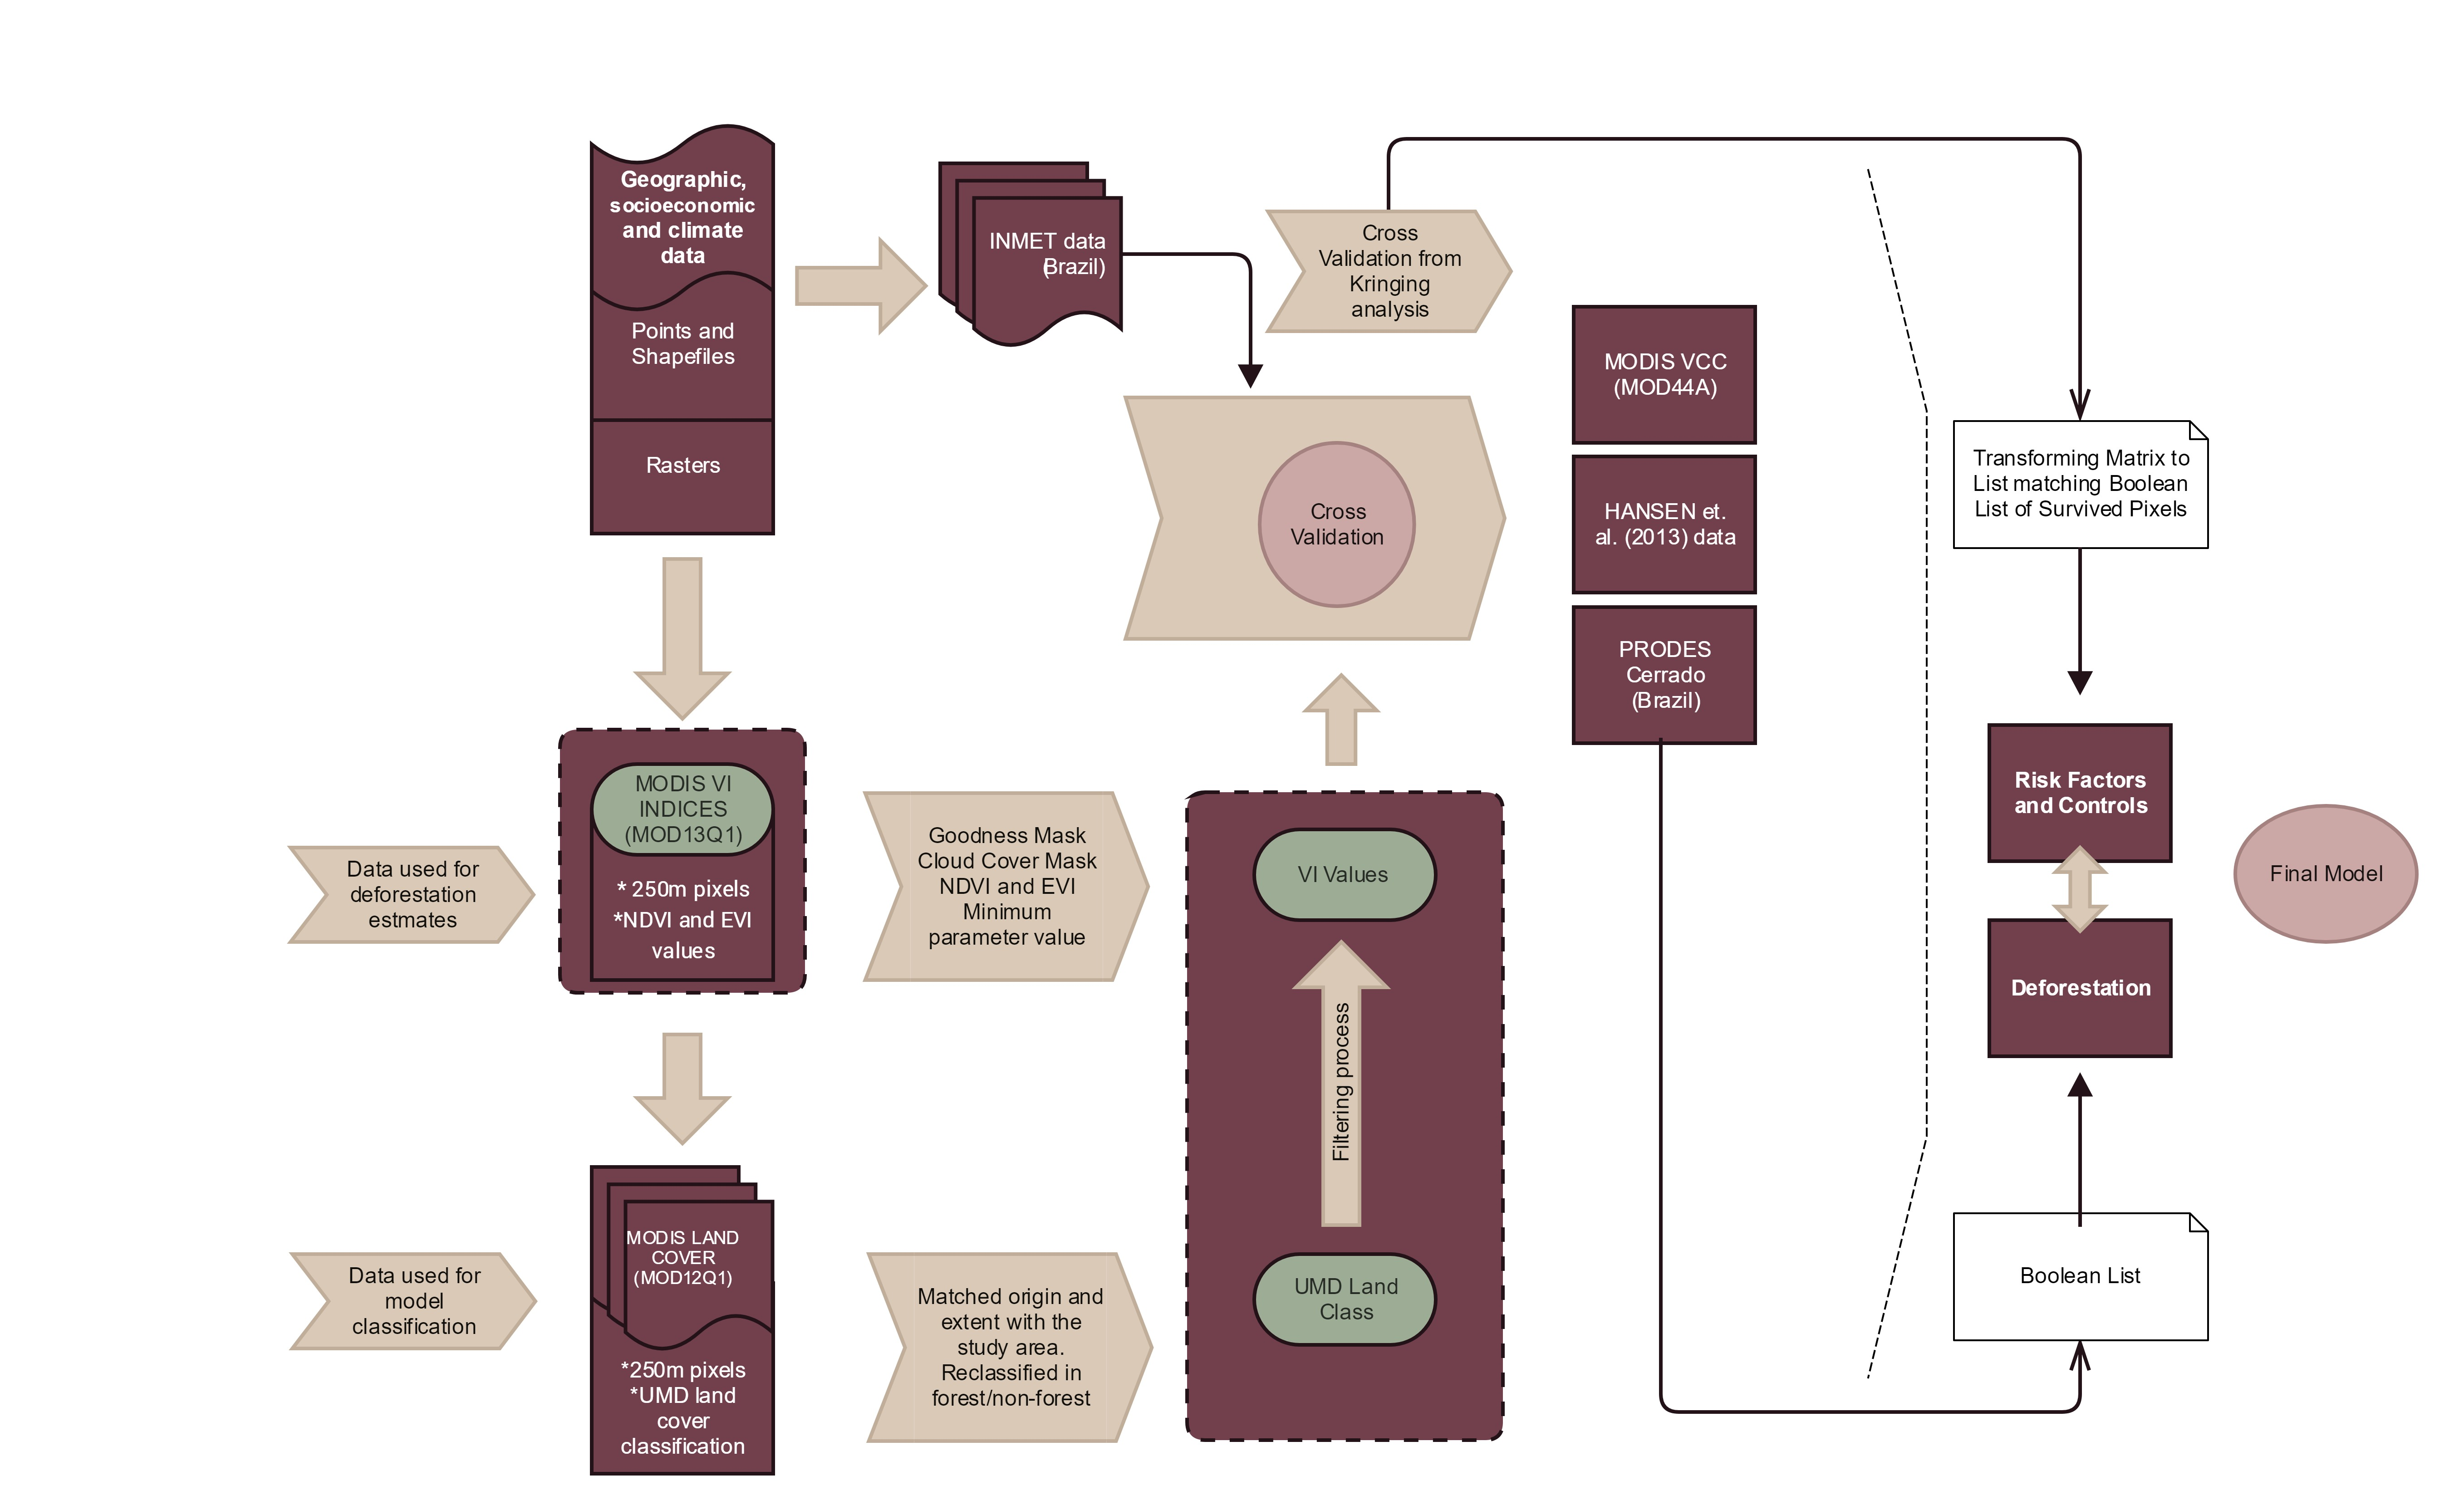
\includegraphics[width=1.5\textwidth]{method.jpg}
\caption{Flowchart of method applied to data. Moving from left to right indicates increasing levels of data processing during the study.}
\label{fig:method}
\end{figure}
\end{landscape}

\begin{table}[H]
\footnotesize
\caption{Model Selection and Validation}
\begin{tabularx}{\linewidth}{X CCCC}
\hline
\hline
Models	& Concordance index & Std Deviation &	K-fold (k=3)	&	Std Deviation \\
\hline
NDVI MA	& 0.767 & 0.001 &	0.30	&	0.0004 \\
NDVI ML	& 0.691 & 0.001	& 0.69	&	0.0008 \\
NDVI Region & 0.755 & 0.001	&	0.03	&	0.0004 \\
EVI MA	& 0.735 & 0.001	& 0.39	&	0.0011 \\
EVI ML & 0.691 & 0.001	&	0.69	&	0.0008 \\
EVI Region & 0.732 & 0.001	&	0.08	&	0.0008 \\
NDVI Sett MA & 0.780 & 0.003 &	0.77	&	0.0040 \\
NDVI Sett ML & 0.798 & 0.003 &	0.79	&	0.0019 \\
NDVI Sett Region & 0.785 & 0.002 &	0.78	&	0.0013 \\
NDVI Buffer MA & 0.582 & 0.005	&	0.58	&	0.0066 \\
NDVI Buffer ML & 0.689 & 0.003	&	0.68	&	0.0052 \\
NDVI Buffer Region & 0.668 & 0.003	&	0.66	&	0.0003 \\
\hline
\hline
\end{tabularx}
\label{kfold}
\end{table}

\begin{table}[H]
\footnotesize
\caption{Descriptive Statistics - Vegetation Indices (Region)}
\begin{tabularx}{\linewidth}{X CCCC}
\hline
\hline
Variables	&	Mean	&	Std Deviation	&	Min	&	Max	 \\
\hline
Period (N)	&	2.653	&	2.628	&	0.000	&	17.000	\\
Censored (N)	&	0.967	&	0.180	&	0.000	&	1.000	\\
Cloud (N)	&	0.711	&	0.453	&	0.000	&	1.000	\\
Period (E)	&	2.459	&	2.344	&	0.000	&	17.000	\\
Censored (E)	&	0.967	&	0.180	&	0.000	&	1.000	\\
Cloud (E)	&	0.711	&	0.453	&	0.000	&	1.000	\\
Lat	&	-2.683	&	0.223	&	-3.064	&	-2.347	\\
Lon	&	-41.892	&	1.171	&	-44.601	&	-39.584	\\
PAs	&	0.539	&	0.355	&	0.000	&	1.228	\\
Mining	&	0.053	&	0.085	&	0.000	&	0.461	\\
Elevation	&	137.934	&	100.009	&	-26	&	993 \\
Markets	&	0.502	&	0.235	&	0.000	&	1.095	\\
Municipalities &	0.128	&	0.058	&	0.000	&	0.341	\\
Rivers	&	0.017	&	0.015	&	0.000	&	0.211	\\
Roads	&	0.037	&	0.037	&	0.000	&	0.218	\\
Region	&	0.404	&	0.491	&	0.000	&	1.000	\\
Neighbours  & 0.992 & 0.161 & 0.000 & 1.000 \\
Rainfall & 130 & 35.695 & 0.000 & 214 \\
Temperature  & 31.7 & 6.241 & 29 & 34 \\
\hline
\hline
\multicolumn{5}{l}{\footnotesize Statistics refer to N=529,680 pixels observations. (N) refers to NDVI and (E) refers to EVI. All distancing }\\
\multicolumn{5}{l}{\footnotesize  values are in decimal degrees. The conversion assumes 0.1 degree to 11km$^{2}$.}
\end{tabularx}
\label{tab:summary}
\end{table}

\begin{table}[H]
\footnotesize
\caption{Descriptive Statistics - Vegetation Indices (MA and LM)}
\begin{tabularx}{\linewidth}{X CCCC}
\hline
\hline
Variables (MA)	&	Mean	&	Std Deviation	&	Min	&	Max	 \\
\hline
Period (N)	&	3.059	&	3.053	&	0.000	&	17.000	\\
Censoring (N)	&	0.956	&	0.205	&	0.000	&	1.000	\\
Clouds (N)	&	0.517	&	0.500	&	0.000	&	1.000	\\
Lat	&	-2.527	&	0.119	&	-2.974	&	-2.347	\\
Lon	&	-41.820	&	1.174	&	-43.980	&	-39.584	\\
Pas	&	0.512	&	0.388	&	0.000	&	1.228	\\
Mining	&	0.065	&	0.098	&	0.000	&	0.461	\\
Elevation	&	123.893	&	87.687	&	-26.000	&	993.000	\\
Markets	&	0.499	&	0.172	&	0.111	&	0.968	\\
Municipalities	&	0.130	&	0.060	&	0.000	&	0.341	\\
Rivers	&	0.017	&	0.016	&	0.000	&	0.211	\\
Roads	&	0.042	&	0.040	&	0.000	&	0.218	\\
Neighbours  & 0.995 &	0.049 &	0.000 &	1.000 \\
Rainfall & 138.9 & 24.877 & 0.000 & 203.000 \\
Temperature  & 32.845 & 1.448 & 29.000 & 34.000 \\
\hline
Variables (LM)	&	Mean	&	Std Deviation	&	Min	&	Max	 \\
\hline
Period (N)	&	2.091	&	1.643	&	0.000	&	17.000	\\
Censoring (N)	&	0.486	&	0.500	&	0.000	&	1.000	\\
Clouds (N)	&	0.941	&	0.235	&	0.000	&	1.000	\\
Lat	&	-2.896	&	0.139	&	-3.064	&	-2.347	\\
Lon	&	-41.987	&	1.134	&	-44.599	&	-39.603	\\
Pas	&	0.580	&	0.310	&	0.000	&	1.227	\\
Mining	&	0.037	&	0.065	&	0.000	&	0.461	\\
Elevation	&	1.542	&	1.094	&	-0.030	&	4.940	\\
Markets	&	0.509	&	0.291	&	0.000	&	1.095	\\
Municipalities	&	0.129	&	0.058	&	0.000	&	0.341	\\
Rivers	&	0.016	&	0.013	&	0.000	&	0.079	\\
Roads	&	0.032	&	0.031	&	0.000	&	0.211	\\
Neighbours	&	0.991	&	0.066	&	0.000	&	1.000	\\
Rainfall	&	116.867	&	44.567	&	0.000	&	214.000	\\
Temperature	&	30.011	&	9.522	&	29.000	&	34.000	\\
\hline
\hline
\multicolumn{5}{l}{\footnotesize Statistics refer to N=529,680 pixels observations. (N) refers to NDVI and (E) refers to EVI. All distancing }\\
\multicolumn{5}{l}{\footnotesize  values are in decimal degrees. The conversion assumes 0.1 degree to 11km$^{2}$.}
\end{tabularx}
\label{tab:summaryMALM}
\end{table}

\begin{landscape}
\begin{table}[H]
\footnotesize
    \caption{Data Description - Sources}
       \begin{tabularx}{0.88\linewidth}{l CXCC}
     \hline
     \hline
       Variable & Source & Description  & Source Data Type & Source Resolution \\
     \hline
    Vegetation Indices & USGS/NASA & Vegetation Index (VI) value at a per pixel basis.  & Raster & 250m \\
    Land Cover & USGS/NASA  & Global land cover types at yearly intervals derived from six different classification schemes. & Raster & 500m\\
    Pas	& MMA & Euclidean distance to nearest protected area in decimal degrees & Polygon & - \\
    Mines & EMBRAPA & Euclidean distance to nearest mineral resource/mining in decimal degrees & Point & -\\
    Elevation & EMBRAPA & Digital elevated map of Maranhao & Raster & 30m\\
    Markets	& CONAB & Euclidean distance to nearest market in decimal degrees & Point & -\\
    Municipalities	& IBGE & Euclidean distance to nearest municipality centre in decimal degrees & Point & -\\
    Rivers	& IBGE & Euclidean distance to nearest river/basin in decimal degrees & Polyline & - \\
    Roads	& IBGE & Euclidean distance to nearest road in decimal degrees & Polyline & - \\
    Settlements & INCRA & Polygons of the settlement areas & Polygon & -\\
    Latitude and Longitude & IBGE & The latitude and longitude of each pixel in the study. This is used to account for spatial autocorrelation across large distances. & Raster & 250m \\
    \hline
    \hline
    \end{tabularx}%
 \label{tab:sources}%
\end{table}%
\end{landscape}